\documentclass[11pt]{article}

\usepackage[margin=1in]{geometry}
\usepackage[T1]{fontenc}
\usepackage{amsmath}
\usepackage{amssymb}
\usepackage{amsthm}
\usepackage{graphicx}
\usepackage{booktabs}
\usepackage{hyperref}

\hypersetup{colorlinks=true, linkcolor=blue, citecolor=blue, urlcolor=blue}

\newtheorem{proposition}{Proposition}

\newcommand{\Var}{\operatorname{Var}}
\newcommand{\Cov}{\operatorname{Cov}}
\newcommand{\dG}{\dim G}

\title{Reconstructing the Gauge Coupling from Gauge-Invariant Entanglement Statistics: The Exactly Solvable Case of Two-Dimensional Yang--Mills}

\author{William T. Trevena\\[3pt]
{\small\itshape Independent Researcher (PhD, ISE, University of Florida)}\\
{\small\texttt{trevenaw7@gmail.com}}}

\date{June 2026}

\begin{document}

\maketitle

{\small\itshape Acknowledgment: Portions of this manuscript were developed with the assistance of Claude (Anthropic), an AI language model, which contributed to literature synthesis, mathematical exposition, drafting, and the computational experiments. Every formula taken from the literature was verified against the arXiv LaTeX source of the cited paper, not from memory; the verification record is \texttt{ym2/FORMULAS.md} in the repository. All numerical claims are reproduced by the published scripts (\texttt{ym2/ym2\_flux.py}, \texttt{ym2/ym2\_su3.py}, deterministic seed 20260609). Consistent with COPE authorship guidelines, the AI system is acknowledged as a tool rather than listed as a coauthor.}

\begin{abstract}
This is the third paper of a series. The first \cite{P1} showed that ``is the coupling hierarchy encoded in vacuum entanglement?'' is ill-posed for frame-dependent entanglement; the second \cite{P2} made the question well-posed algebraically and answered it negatively in the minimal toy, where all gauge-invariant entanglement is the classical edge (center) term. This paper presents the positive case the no-gos point to: the one setting where gauge-field entanglement is exactly computable and purely edge --- two-dimensional Yang--Mills on a sphere --- and where the coupling is not merely reflected in invariant entanglement data but \emph{efficiently estimable} from it. For compact gauge group $G$ in the Hartle--Hawking state, the boundary-flux distribution $p_R(t) \propto (\dim R)^2 e^{-(t/2)C_2(R)}$, $t = g^2 A$, is a one-parameter exponential family, which yields three exact statements: (i) $dS/dt = -(t/4)\Var_t(C_2) < 0$ --- the entanglement entropy is strictly decreasing in the coupling, so $t \mapsto S(t)$ is a bijection; (ii) the Fisher information of the flux measurement is $I(t) = \tfrac14\Var_t(C_2)$, so entropy susceptibility and statistical reconstructability are the same function, $dS/dt = -t\,I(t)$; (iii) the capacity of entanglement is $C(t) = t^2 I(t) \to \tfrac12\dG$ as $t \to 0$. Maximum-likelihood reconstruction from $N$ flux samples saturates the Cram\'er--Rao bound for $\mathrm{U}(1)$, $\mathrm{SU}(2)$, and $\mathrm{SU}(3)$ --- the gauge group of QCD: at $t = 1$, the coupling is recovered to $1.6\%$ from $10^3$ samples and $0.5\%$ from $10^4$. With $n$ intervals the entropy grows linearly in $n$ through the edge term $2n\langle \ln \dim R\rangle$, but the Fisher information does not grow at all: the flux at every cut is one global random variable, so entropy scales while information does not. We state precisely why all of this demonstrates \emph{reflection}, not determination: the inference inverts a known one-parameter family; only the product $g^2 A$ is recoverable; the edge term that carries it is contested as entanglement; and the one sharp $d = 4$ computation in the literature has the coupling dropping out. The open question the series leaves is whether any $d = 4$ analog of this $d = 2$ encoding exists.
\end{abstract}

\section{Introduction}

\subsection{The series}

This paper completes an arc that began with a question and ends with the only version of an affirmative answer we believe the current literature supports.

\textbf{Paper 1} \cite{P1} asked whether the Standard Model coupling hierarchy is encoded in the entanglement entropies of a three-qubit vacuum state, and answered with no-go results: the static matching problem is underconstrained (any hierarchy can be matched; matching is non-evidential), and --- the diagnosis that drives everything after it --- the question is \emph{ill-posed}, because gauge transformations act on fermionic modes rather than on qubit tensor factors, so the entanglement entropies in question are gauge-frame dependent (\cite{P1}, Sec.~9.3).

\textbf{Paper 2} \cite{P2} made the question well-posed by replacing subsystem entropies with entanglement relative to the gauge-invariant operator algebra (Barnum--Knill--Ortiz--Viola \cite{BKOV}; Zanardi \cite{Zanardi}; in the gauge-field form, Casini--Huerta--Rosabal \cite{CHR}) and computed the answer exactly in the minimal toy. The well-posed answer was a sharper no-go: the single-copy invariant data is the charge-sector distribution alone; the quantum piece of the algebraic entropy vanishes identically for every pure state (``all edge, no bulk''); and the one static ``match'' of Paper 1 turned out to be pure gauge.

Both papers end at the same object from opposite sides: the \emph{classical center/edge term} of gauge-invariant entanglement --- the Shannon entropy of the boundary-flux distribution. Paper 2 showed it is the only gauge-invariant entanglement there is in the toy. The verified literature review accompanying the series showed it is the only place a gauge coupling demonstrably enters entanglement in low dimensions. The natural final question is therefore: \textbf{in the best possible case, how much of the coupling does the invariant edge data actually carry, and how efficiently can it be extracted?}

\textbf{This paper} answers that question in the one setting where it is exactly solvable: pure Yang--Mills theory in two spacetime dimensions.

\subsection{The honest thesis}

Our thesis has a positive half and a deflationary half, and we state both up front.

\emph{Positive.} In 2d Yang--Mills on a sphere (Hartle--Hawking state, compact group $G$), the gauge-invariant entanglement data of an interval --- the distribution $p_R(t)$ of the boundary electric flux, and the entanglement entropy $S(t)$ built from it --- determines the dimensionless coupling $t = g^2 A$ \textbf{exactly and efficiently}: $S(t)$ is strictly decreasing (an identity, not a numerical observation), so the map $t \mapsto S$ is a bijection; and an observer who measures the flux $N$ times can estimate $t$ with the smallest variance allowed by statistics, saturating the Cram\'er--Rao bound, because the flux distribution is an exponential family in the coupling. This includes $G = \mathrm{SU}(3)$: in the $d = 2$ world, the gauge coupling of the strong interaction is reconstructible from gauge-invariant entanglement statistics, and more efficiently than for smaller groups.

\emph{Deflationary.} This demonstrates \textbf{reflection, not determination}. The inference presupposes the theory --- the group, the state preparation, the known one-parameter family $p_R(t)$ --- and recovers the value of a parameter the family was already known to depend on. It does not show that the coupling is \emph{constituted by} entanglement, nor that any of this survives to $d = 4$, where the only sharp computation of a coupling-sensitive entanglement coefficient finds it independent of the coupling's value \cite{CHMP}. Section~\ref{sec:scope} makes the deflation precise; Section~\ref{sec:d34} prices out what $d = 3$ and $d = 4$ would require.

The series, in one line: Papers 1--2 eliminated the frame-dependent encodings; this paper exhibits, and quantifies to the statistical limit, the invariant encoding that actually exists in $d = 2$.

\subsection{Contributions}

Each contribution carries an epistemic label, as throughout the series. ``Literature-verified'' means checked against the arXiv LaTeX source of the cited paper (record: \texttt{ym2/FORMULAS.md}). ``Derived'' means proven here from literature-verified formulas (the proofs are short and given in full). ``Computed'' means machine-verified by the published deterministic scripts.

\begin{enumerate}

\item \textbf{Monotonicity theorem} (derived; computed to stated residuals). For any compact $G$, the interval entanglement entropy of the Hartle--Hawking state obeys $dS/dt = -(t/4)\Var_t(C_2) < 0$ on $t \in (0,\infty)$; hence $t \mapsto S(t)$ is a smooth bijection $(0,\infty) \to (0,\infty)$ and the coupling is recoverable from the exact entropy. Numerical inversion recovers $t$ to $\leq 9\times10^{-14}$ across three groups (Sec.~\ref{sec:mono}).

\item \textbf{Fisher-information identity and Cram\'er--Rao saturation} (derived; computed). The flux distribution is a one-parameter exponential family with sufficient statistic $C_2(R)$; its Fisher information is $I(t) = \tfrac14\Var_t(C_2)$, so $dS/dt = -t\,I(t)$: the entropy's sensitivity to the coupling \emph{is} ($t$ times) the statistical information the flux carries about the coupling. Maximum-likelihood estimation from $N$ flux samples saturates the Cram\'er--Rao bound for $\mathrm{U}(1)$, $\mathrm{SU}(2)$, $\mathrm{SU}(3)$ (Sec.~\ref{sec:recon}).

\item \textbf{SU(3) --- the QCD group} (computed; new in this paper). The analysis extends to $\mathrm{SU}(3)$ with irreps $(p,q)$, $\dim = (p+1)(q+1)(p+q+2)/2$, $C_2 = (p^2+q^2+pq+3p+3q)/3$ (convention verified, Sec.~\ref{sec:groupdata}). At $t = 1$ the coupling is recovered to $1.6\%$ from $10^3$ samples, $0.5\%$ from $10^4$, at Cram\'er--Rao efficiency ${\sim}1.0$. Reconstruction \emph{improves} with group size: $I(t) \to \dG/(2t^2)$ at weak coupling, so the larger the gauge group, the more information each flux sample carries (Sec.~\ref{sec:qcd}).

\item \textbf{Capacity of entanglement} (derived; computed). $C(t) \equiv \Var(-\ln\rho) = t^2 I(t)$, with $C(t) \to \tfrac12\dG$ as $t \to 0$ (verified to $10^{-6}$ at $t = 0.05$ for all three groups). We found no prior computation of the capacity of entanglement in 2d Yang--Mills (search record in the companion notes); the concept is due to Yao--Qi \cite{YQ10} and was developed in QFT by de Boer--J\"arvel\"a--Keski-Vakkuri \cite{dBJK18} (Sec.~\ref{sec:capacity}).

\item \textbf{$n$ intervals: entropy scales, information does not} (derived; computed; the qualitative point is Donnelly's \cite{D14}). For a region of $n$ intervals the entropy is $S_n = H[p] + 2n\langle\ln d\rangle$ \cite[eq.~(YM2entropy), literature-verified]{D14}, and we derive $dS_n/dt = -(t/4)\Var(C_2) - (n-1)\Cov(\ln d, C_2)$, strictly negative for all $n$ in all cases computed. But the flux variables at the $2n$ cut points are \emph{perfectly correlated} --- one global $R$ --- so the Fisher information is exactly $n$-independent: more cuts give no new information about the coupling, and a numerical experiment confirms the estimator obeys the $N$-preparation bound, not the hypothetical $2nN$-sample bound (Sec.~\ref{sec:ncuts}). 2d Yang--Mills's flux is one global random variable; the edge entropy counts cut points, not information.

\item \textbf{Scope, stated as sharply as the results} (literature-verified). Everything here is $d = 2$ and purely the contested edge term; only the product $g^2 A$ is recoverable; and the $d = 4$ evidence runs \emph{against} naive extrapolation (Secs.~\ref{sec:scope}--\ref{sec:d34}).

\end{enumerate}

\section{Setting and Verified Formulas}\label{sec:setting}

\textbf{Status: literature-verified (sources and verbatim strings in \texttt{ym2/FORMULAS.md}).}

\subsection{The theory and the state}

Pure Yang--Mills theory with compact gauge group $G$ in two Euclidean dimensions is exactly solvable: the heat-kernel lattice action is self-reproducing under plaquette merging, so every amplitude on every surface has a closed form as a sum over irreps \cite{Mig75, Rus90, Wit91, CMR94}. On a closed surface $\Sigma$ of area $V$ and Euler characteristic $\chi$,
\[
Z(\Sigma) = \sum_R (\dim R)^{\chi}\, \exp\!\left[-\tfrac{g^2 V}{2}\, C_2(R)\right],
\]
with $C_2$ the quadratic Casimir. The theory has no propagating degrees of freedom; by invariance under area-preserving diffeomorphisms, $g^2$ and the areas enter only through products $g^2 \cdot (\text{area})$.

The state is the \textbf{Hartle--Hawking (sphere) state} on a spatial circle, the setting of Donnelly's nonabelian analysis \cite{D14}: the wavefunction prepared by the path integral over a hemisphere (disk) of area $A/2$,
\[
\psi(R) \propto (\dim R)\, e^{-(g^2 A/4)\, C_2(R)},
\]
expressed in the character basis $|R\rangle$ of the physical Hilbert space (class functions of the circle holonomy). Everything depends on the single dimensionless parameter
\[
t \equiv g^2 A, \qquad A = \text{total sphere area} \qquad (g^2 \text{ has dimension } 1/\text{area in } d = 2).
\]

\subsection{The two formulas}\label{sec:formulas}

Cutting the circle into a region $A$ of $n$ disjoint intervals ($2n$ cut points) and embedding into the extended Hilbert space (one copy of $L^2(G)$ per interval), the reduced density matrix is block-diagonal in the boundary irrep $R$ (``electric flux''), with each block maximally mixed over the edge multiplicity space of dimension $(\dim R)^{2n}$ \cite{D14} (for the extended-Hilbert-space construction in general lattice gauge theories see also \cite{D11, GST15}). The two formulas everything in this paper rests on are:

\textbf{(F1) Flux distribution} \cite[eq.~(pr)]{D14}:
\begin{equation}\label{eq:flux}
p_R(t) = \frac{d_R^2\, e^{-(t/2)C_2(R)}}{Z(t)}, \qquad Z(t) = \sum_R d_R^2\, e^{-(t/2)C_2(R)},
\end{equation}
where $d_R = \dim R$. This is the probability of measuring boundary flux $R$ at the cut --- in 2d YM, the Casimir of the boundary electric field is the \emph{only} local gauge-invariant observable \cite{D14}. Note that $p_R$ does not depend on $n$ (Sec.~\ref{sec:ncuts}).

\textbf{(F2) Entanglement entropy, $n$ intervals} \cite[eq.~(YM2entropy)]{D14}; verbatim from the source: \verb|S = \sum_R p(R) (- \log p(R) + 2n \log \dim R)|:
\begin{equation}\label{eq:Sn}
S_n(t) = -\sum_R p_R \ln p_R + 2n \sum_R p_R \ln d_R = H[p(t)] + 2n\langle \ln d\rangle_t.
\end{equation}
The same result follows from the Euclidean replica trick on the sphere with $n$ cuts (Gromov--Santos \cite[eq.~(answ)]{GS14}, $\chi = 2$, $l = n$; the $l = 1$, $v = 0$ special case was obtained earlier by Velytsky \cite{V08}), up to the additive counterterm discussed below. We use $n = 1$ except in Sec.~\ref{sec:ncuts}. In the three-term decomposition of \cite{D11}, the first term of \eqref{eq:Sn} is the classical (Shannon) piece, the second is the boundary log-dim piece, and the third term --- distillable ``nonlocal correlations'' --- \textbf{vanishes identically}: the entropy is entirely the edge/center term (see also the path-integral edge-mode treatment of \cite{BMV18}). This is the field-theory realization of the ``all edge, no bulk'' structure computed in the toy of \cite{P2}.

\subsection{Group data and conventions}\label{sec:groupdata}

\begin{center}
\begin{tabular}{llll}
\toprule
$G$ & irreps $R$ & $\dim R$ & $C_2(R)$ \\
\midrule
compact $\mathrm{U}(1)$ & $n \in \mathbb{Z}$ & $1$ & $n^2$ \\
$\mathrm{SU}(2)$ & $j \in \{0, \tfrac12, 1, \dots\}$ & $2j+1$ & $j(j+1)$ \\
$\mathrm{SU}(3)$ & $(p,q)$, $p,q \in \mathbb{Z}_{\geq 0}$ & $(p+1)(q+1)(p+q+2)/2$ & $(p^2+q^2+pq+3p+3q)/3$ \\
\bottomrule
\end{tabular}
\end{center}

\textbf{SU(3) convention (verified against standard sources, June 2026 \cite{su3data}).} The Dynkin-label formulas above give $C_2(1,0) = 4/3 = (N^2-1)/2N$ for the fundamental and $C_2(1,1) = 3 = N$ for the adjoint --- the normalization in which $\operatorname{Tr}(T_a T_b) = \tfrac12\delta_{ab}$ in the fundamental. This is the same family as $C_2(j) = j(j+1)$ for $\mathrm{SU}(2)$ (fundamental: $3/4 = (N^2-1)/2N$) and matches the convention of \cite{D14}. Both formulas are asserted at runtime in \texttt{ym2\_su3.py} on the low-lying irreps ($\mathbf{1} = (0,0)$, $\mathbf{3} = (1,0)$, $\bar{\mathbf{3}} = (0,1)$, $\mathbf{6} = (2,0)$, $\mathbf{8} = (1,1)$, $\mathbf{10} = (3,0)$). Any rescaling $C_2 \to \kappa C_2$ --- e.g., the 't~Hooft-style convention of \cite{GS14}, which is $2\times$ ours for $\mathrm{SU}(2)$ --- is the reparametrization $t \to \kappa t$ and changes nothing structural.

\textbf{Additive ambiguity.} $S$ carries a $t$-\emph{independent} additive ambiguity: the local counterterm $2lv$ of \cite{GS14}, the measure/bare-action constant footnoted in \cite{D14}, the center-choice ambiguity of \cite{CHR}. We fix it by the extended-Hilbert-space counting (trivial flux sector nondegenerate; $S \to 0$ as $t \to \infty$). The distribution $p_R(t)$ and all $t$-derivatives of $S$ are ambiguity-free, and the reconstruction below uses only those.

\section{Exact Results}\label{sec:exact}

\subsection{Exponential-family structure}

\textbf{Status: derived (elementary); the observation that drives the paper.}

Eq.~\eqref{eq:flux} is a one-parameter exponential family in $\theta = -t/2$ with sufficient statistic $C_2(R)$ and base measure $d_R^2$. Writing $\langle\cdot\rangle$, $\Var$, $\Cov$ for moments under $p(t)$, the standard cumulant identities give
\begin{equation}\label{eq:cumulant}
\frac{d\langle f(R)\rangle}{dt} = -\tfrac12 \Cov_t(f, C_2) \quad \text{for any statistic } f, \qquad \frac{d \ln Z}{dt} = -\tfrac12\langle C_2\rangle.
\end{equation}
Everything in Secs.~\ref{sec:mono}--\ref{sec:ncuts} is a corollary of \eqref{eq:cumulant}.

\subsection{Monotonicity: \texorpdfstring{$S$ determines $t$}{S determines t}}\label{sec:mono}

\textbf{Status: derived; computed (machine-verified residuals quoted).}

From \eqref{eq:flux}, the eigenvalues of the reduced density matrix in flux sector $R$ ($n = 1$) are $\lambda_R = e^{-(t/2)C_2(R)}/Z$, each $d_R^2$-fold degenerate, so $-\ln\lambda_R = \ln Z + (t/2)C_2(R)$ and
\begin{equation}\label{eq:SlnZ}
S(t) = \ln Z(t) + \tfrac{t}{2}\langle C_2\rangle_t.
\end{equation}
Differentiating with \eqref{eq:cumulant}:

\begin{proposition}[monotonicity]\label{prop:mono}
For any compact $G$,
\begin{equation}\label{eq:dSdt}
\frac{dS}{dt} = -\tfrac12\langle C_2\rangle + \tfrac12\langle C_2\rangle + \tfrac{t}{2}\left(-\tfrac12\Var_t(C_2)\right) = -\frac{t}{4}\,\Var_t(C_2) \;<\; 0
\end{equation}
for all $t > 0$, since $p(t)$ has full support on irreps with distinct Casimirs. $Z(t)$ is analytic on $(0,\infty)$, so $S$ is smooth and strictly decreasing, with $S \to \infty$ as $t \to 0^+$ and $S \to 0$ as $t \to \infty$: the map $t \mapsto S(t)$ is a bijection $(0,\infty) \to (0,\infty)$. The dimensionless coupling $t = g^2 A$ is exactly recoverable from the entanglement entropy.
\end{proposition}

\emph{Computed verification.} On $t \in [0.05, 20]$ (400-point geometric grid): $S$ strictly decreasing for $\mathrm{U}(1)$, $\mathrm{SU}(2)$, $\mathrm{SU}(3)$; the analytic derivative \eqref{eq:dSdt} matches finite differences to better than $0.3\%$ ($\mathrm{SU}(2)$, $\mathrm{U}(1)$) and $0.6\%$ ($\mathrm{SU}(3)$) everywhere on the grid (grid-stencil error), and to $2.4\times10^{-10}$ with dedicated central differences (Sec.~\ref{sec:ncuts}); max $dS/dt$ on the grid: $-6.2\times10^{-3}$ ($\mathrm{SU}(2)$), $-4.5\times10^{-4}$ ($\mathrm{U}(1)$), $-2.6\times10^{-4}$ ($\mathrm{SU}(3)$) --- bounded away from zero. Practical inversion (given exact $S$, root-find $t$) recovers $t$ to $\leq 9\times10^{-14}$ at six test points per group. The Shannon-only piece $H(t) = S - 2\langle\ln d\rangle$ is \emph{not} manifestly monotonic ($dH/dt = -(t/4)\Var(C_2) + \Cov(\ln d, C_2)$, a competition); numerically it is also strictly decreasing for all three groups on the grid, but only the full $S$ has the analytic proof. We flag this honestly because $H$, not $S$, is the piece \cite{D14} identifies with uncertainty in gauge-invariant observables.

The weak-coupling behavior is universal, and it is what justifies $S \to \infty$ in Proposition~\ref{prop:mono}: $Z(t) = \sum_R d_R^2 e^{-(t/2)C_2(R)}$ is the heat kernel of the group manifold $G$ evaluated at the identity, whose short-time behavior is the standard flat divergence $Z(t) \simeq \mathrm{vol}(G)\,(2\pi t)^{-\dG/2}$ \cite{Cam90, CMR94}, so $S \simeq \tfrac12\dG\,\ln(1/t) + \text{const}$ as $t \to 0$. Computed witness: $S(t) + \tfrac12\dG\,\ln t$ is constant to better than $10^{-6}$ over $t \in [0.002, 0.2]$ for all three groups, and for $\mathrm{U}(1)$ the constant equals the exact heat-kernel value $\tfrac12 + \tfrac12\ln 2\pi = 1.4189385$ to seven digits. This is consistent with the weak-coupling scaling of \cite{GS14}, and formally the same $\tfrac12\dG\,\log(\text{coupling})$ structure as Radi\v{c}evi\'c's $d = 3$ universal term \cite{R15}.

\subsection{Fisher information: reconstructability = susceptibility}\label{sec:fisher}

\textbf{Status: derived; the framing we believe is new (novelty scan in the companion notes).}

For the family \eqref{eq:flux}, $\partial_t \ln p_R = \tfrac12(\langle C_2\rangle - C_2(R))$, so the Fisher information of one flux measurement is
\begin{equation}\label{eq:fisher}
I(t) = \mathbb{E}\!\left[(\partial_t \ln p_R)^2\right] = \tfrac14\,\Var_t(C_2),
\end{equation}
and the Cram\'er--Rao bound for any unbiased estimator of $t$ from $N$ i.i.d.\ flux samples is $\Var(\hat t) \geq 1/(N I(t)) = 4/(N \Var_t(C_2))$. Comparing \eqref{eq:dSdt} and \eqref{eq:fisher}:
\begin{equation}\label{eq:dSisI}
\boxed{\;\frac{dS}{dt} = -t\, I(t).\;}
\end{equation}
The entropy's sensitivity to the coupling and the statistical information the flux carries about the coupling are the same function of $t$, up to the factor $-t$. Physically, $\Var_t(C_2)$ is the flux susceptibility of the vacuum --- the object the synthesis of this series identified as ``the defensible core'' of any coupling-from-entanglement claim. Eq.~\eqref{eq:dSisI} says that in $d = 2$ the identification is exact: \emph{entanglement susceptibility is Fisher information.}

\emph{The flux measurement is quantum-optimal.} A referee may ask whether some other measurement on the interval extracts more information about $t$. No: the reduced density matrices $\{\rho_A(t)\}$ are all diagonal in the same flux-block basis (eq.~\eqref{eq:flux} with $t$-independent eigenvectors), so the family is mutually commuting, and the quantum Fisher information of $\rho_A(t)$ equals the classical Fisher information of its eigenvalue distribution \cite{BC94}. Within a block the state is maximally mixed with $t$-independent weights $1/d_R^2$, carrying no information; the eigenvalue distribution over blocks is $p_R(t)$. Hence $\mathrm{QFI}(t) = I(t) = \tfrac14\Var_t(C_2)$: the flux measurement saturates the quantum Cram\'er--Rao bound among all measurements on the interval's algebra, and \eqref{eq:fisher} is not an artifact of a convenient measurement choice.

\subsection{Capacity of entanglement}\label{sec:capacity}

\textbf{Status: derived; computed. Concept from \cite{YQ10, dBJK18}; we found no prior YM$_2$ appearance.}

The capacity of entanglement is the variance of the modular Hamiltonian, $C(t) \equiv \Var(-\ln\rho_A)$ --- the entanglement analog of heat capacity \cite{YQ10, dBJK18}. Since $-\ln\lambda_R = \ln Z + (t/2)C_2(R)$ is affine in $C_2$,
\begin{equation}\label{eq:capacity}
C(t) = \tfrac{t^2}{4}\,\Var_t(C_2) = t^2\, I(t), \qquad \text{and} \qquad \frac{dS}{dt} = -\frac{C(t)}{t}.
\end{equation}
In this model the capacity of entanglement \emph{is} the Fisher information in disguise --- a clean instance of the thermodynamic analogy (capacity $\leftrightarrow$ heat capacity $\leftrightarrow$ fluctuation $\leftrightarrow$ information) becoming an identity. Computed: $C(t) \to \tfrac12\dG$ as $t \to 0^+$, equal to $0.5000$, $1.5000$, $4.0000$ ($\mathrm{U}(1)$, $\mathrm{SU}(2)$, $\mathrm{SU}(3)$) at $t = 0.05$ to the precision quoted in the results files; equivalently $S \simeq \tfrac12\dG\,\ln(1/t)$ at weak coupling, with the capacity plateau ending around $t \sim 1$ ($\mathrm{SU}(3)$ still $3.995$ at $t \approx 3.9$).

\emph{Prior work.} Capacity of entanglement was introduced in \cite{YQ10}, studied systematically in QFT and holography in \cite{dBJK18}, and computed for local-operator excitations of 4d free Yang--Mills in \cite{N21}. We also note the contact with the symmetry-resolved entanglement literature: the flux-block decomposition of $\rho_A$ is precisely a charge/sector-resolved structure in the sense of \cite{GS18, XAS18}, and the capacity of entanglement has been used as a probe of RG flows and symmetry resolution in \cite{ADKT23}; our eq.~\eqref{eq:capacity} is the YM$_2$ instance in which the sector distribution alone carries all of the $t$-dependence. Searches (June 2026; queries recorded in the companion notes) found no prior computation in 2d Yang--Mills and no prior statement of \eqref{eq:fisher}--\eqref{eq:capacity} there; we flag that the entanglement entropy of YM$_2$ itself is thoroughly studied \cite{GS14, D14, DTV19, MOPT26}, so \eqref{eq:capacity} is best read as low-hanging fruit made visible by the Fisher framing, not as a difficult result.

\subsection{\texorpdfstring{$n$}{n} intervals: the entropy scales, the information does not}\label{sec:ncuts}

\textbf{Status: formula \eqref{eq:Sn} literature-verified; identity \eqref{eq:dSndt} derived; non-scaling of information derived and computed; the qualitative point is already in \cite{D14}.}

\emph{Setting adopted (stated carefully, since the cut topology matters).} The spatial manifold is the circle in the HH sphere state; region $A$ = $n$ disjoint intervals, complement = $n$ intervals, $2n$ cut points. The physical state is a class function of the single circle holonomy, $\psi = \sum_R c_R |R\rangle$; iterating Donnelly's embedding map, the character state $|R\rangle$ embeds into the $2n$-interval extended Hilbert space with one $d_R$-dimensional index pair per cut point, all carrying the \emph{same} $R$. The reduced density matrix is therefore block-diagonal in \textbf{one global flux label $R$} with the \emph{$n$-independent} distribution $p_R(t)$ of eq.~\eqref{eq:flux}, each block maximally mixed of dimension $d_R^{2n}$. This yields \eqref{eq:Sn}, whose log-dim term ``appears once for each of the $2n$ points on the boundary of $A$'' \cite[verbatim]{D14}. The replica computation of \cite{GS14} on the sphere with $l = n$ cuts gives the same $t$-dependence. (On higher-genus surfaces or for non-HH states the sector structure is richer \cite{MOPT26}; we do not use those settings.)

\emph{Entropy.} From $S_n = S_1 + 2(n-1)\langle\ln d\rangle$ and \eqref{eq:cumulant}:
\begin{equation}\label{eq:dSndt}
\frac{dS_n}{dt} = -\frac{t}{4}\,\Var_t(C_2) - (n-1)\,\Cov_t(\ln d, C_2).
\end{equation}
Computed: \eqref{eq:dSndt} matches central finite differences to $\leq 2.4\times10^{-10}$ relative over 48 (group, $t$, $n$) combinations ($\mathrm{U}(1)$, $\mathrm{SU}(2)$, $\mathrm{SU}(3)$; $t \in \{0.3, 1, 3, 8\}$; $n \in \{1,2,3,4\}$). $\Cov_t(\ln d, C_2) > 0$ on the full 400-point grid for $\mathrm{SU}(2)$ and $\mathrm{SU}(3)$ (minima $1.1\times10^{-3}$ and $4.3\times10^{-5}$ respectively) and is identically $0$ for $\mathrm{U}(1)$ ($d \equiv 1$); so $S_n$ is strictly decreasing in $t$ for every $n$ in all cases computed --- each additional pair of cut points makes the entropy \emph{more} coupling-sensitive, by $(n-1)\Cov$.

\emph{Information.} Does Fisher information scale with $n$ --- do more cuts mean more flux samples? \textbf{No.} The $2n$ cut-point fluxes of one prepared circle are copies of the single global $R$: perfectly correlated, joint distribution supported on the diagonal with weights $p_R(t)$. The Fisher information of the joint measurement is therefore exactly $I(t) = \tfrac14\Var_t(C_2)$, independent of $n$. Donnelly states the qualitative point verbatim for the abelian case \cite{D14}: ``the entropy is independent of the number of intervals traced out\dots\ Having access to an additional interval therefore does not change the amount of information one can acquire about the state.'' (In the nonabelian case the \emph{entropy} does grow with $n$ --- but only through the $2n\langle\ln d\rangle$ edge term, which \cite{D14} notes ``is not associated to uncertainty in gauge-invariant observables.'')

\emph{Computed demonstration.} $M = 400$ trials, each preparing $N = 1000$ independent circles cut into $n = 3$ intervals (6 cut points, 6000 flux readings, 1000 independent values). The MLE from the 6000-reading dataset is \emph{identical} to the MLE from the 1000 unique samples (duplication leaves the sufficient statistic unchanged; verified to $10^{-14}$ relative, exact as estimators), and its standard deviation matches the $N$-preparation Cram\'er--Rao bound, not the hypothetical $2nN$-sample bound: $\mathrm{sd}/\mathrm{CRB}_N = 0.93$ ($\mathrm{SU}(3)$), $0.97$ ($\mathrm{SU}(2)$); $\mathrm{sd}/\mathrm{CRB}_{2nN} = 2.27$, $2.37 \approx \sqrt{6}\cdot(\mathrm{sd}/\mathrm{CRB}_N)$.

The moral is worth the sentence: \textbf{in 2d Yang--Mills, entropy counts cut points; information counts independent preparations.} The edge term $2n\langle\ln d\rangle$ --- the dominant part of $S_n$ for large $n$ --- carries no additional information about the coupling beyond what one cut already provides. A referee who suspects that ``more entanglement entropy'' must mean ``better reconstruction'' has it exactly backwards here, and the structure of the reduced state says why: 2d YM's flux is one global random variable. (Compare the flux-tube entanglement of \cite{ASV24}, which likewise depends on the number of boundary crossings and $\dim R$ but not on lengths.)

\begin{figure}[t]
\centering
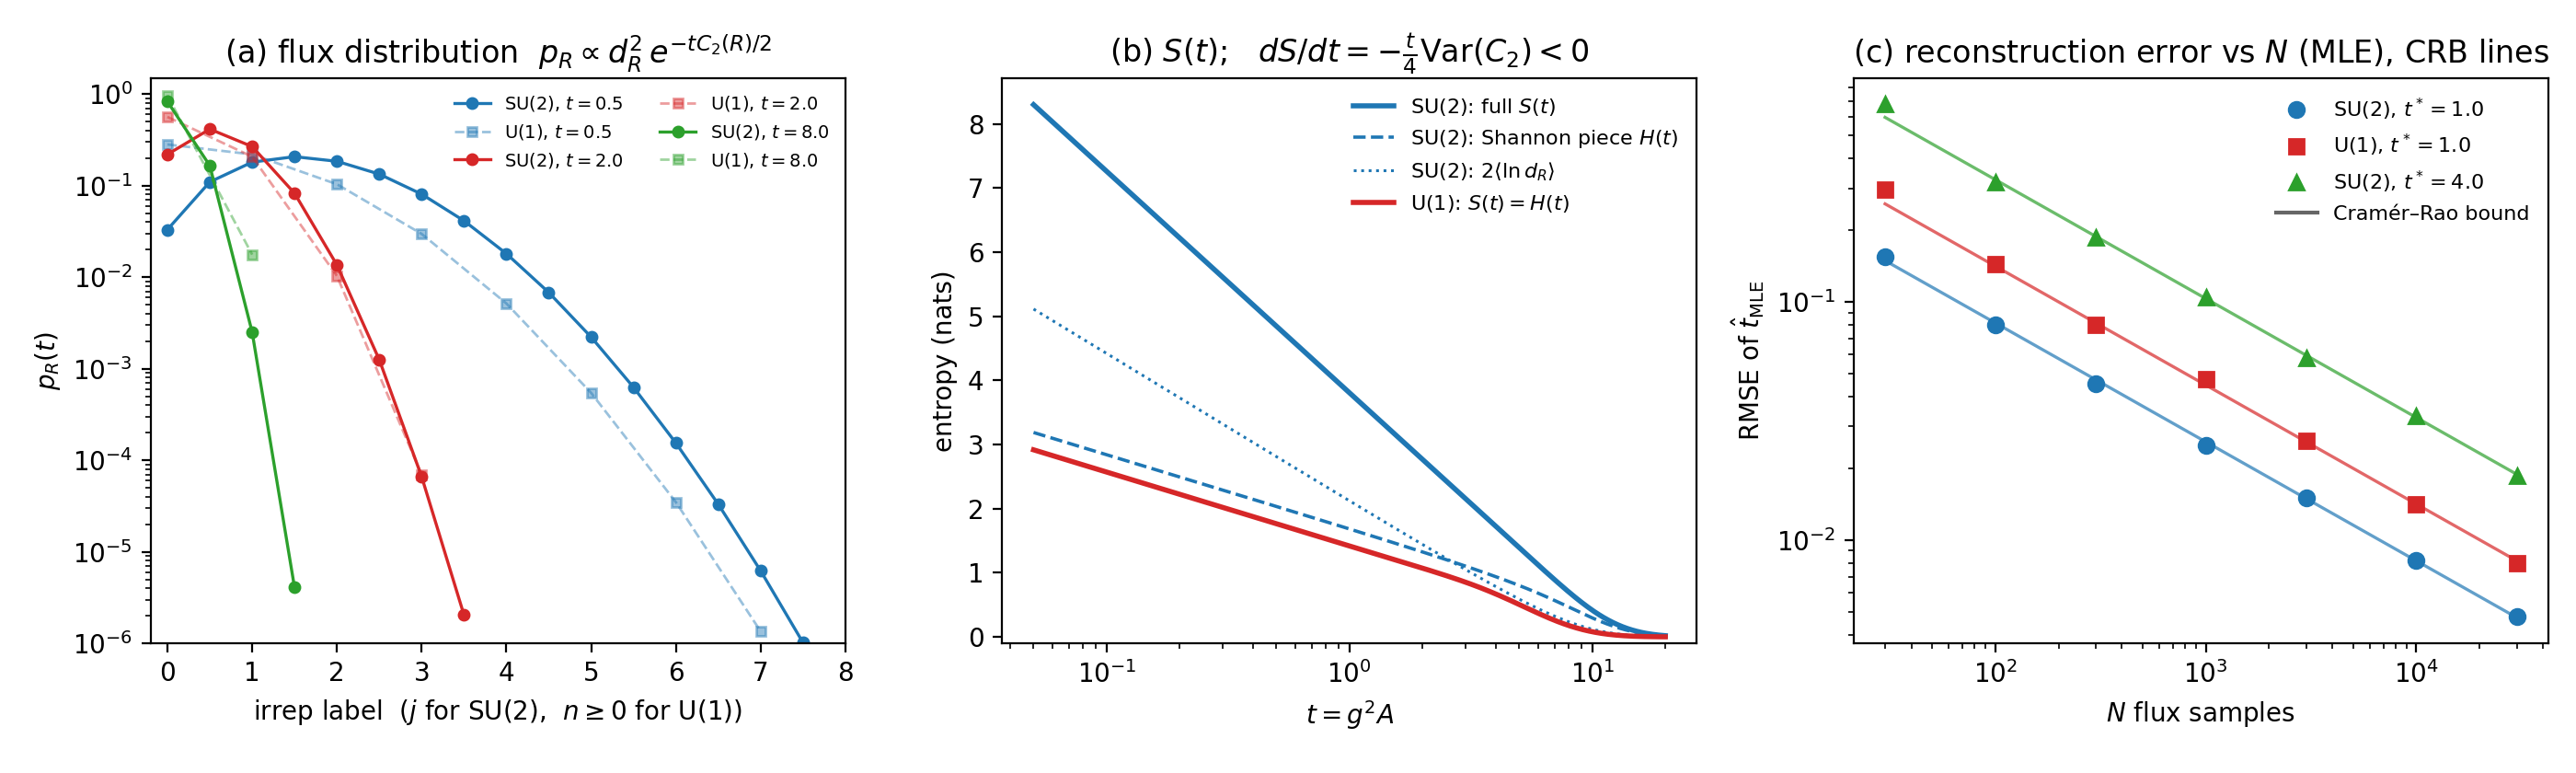
\includegraphics[width=\textwidth]{fig_ym2.png}
\caption{$\mathrm{U}(1)$ and $\mathrm{SU}(2)$ (script \texttt{ym2\_flux.py}, seed 20260609). (a)~Flux distribution $p_R(t)$ of eq.~\eqref{eq:flux} at $t \in \{0.5, 2, 8\}$. (b)~Entropy $S(t)$, its Shannon piece $H(t)$, and the edge term: all strictly decreasing, Proposition~\ref{prop:mono}. (c)~RMSE of the maximum-likelihood estimate $\hat t$ versus number of flux samples $N$, against the Cram\'er--Rao lines $\sqrt{1/(N I(t^*))}$ (Sec.~\ref{sec:results}).}
\label{fig:ym2}
\end{figure}

\begin{figure}[t]
\centering
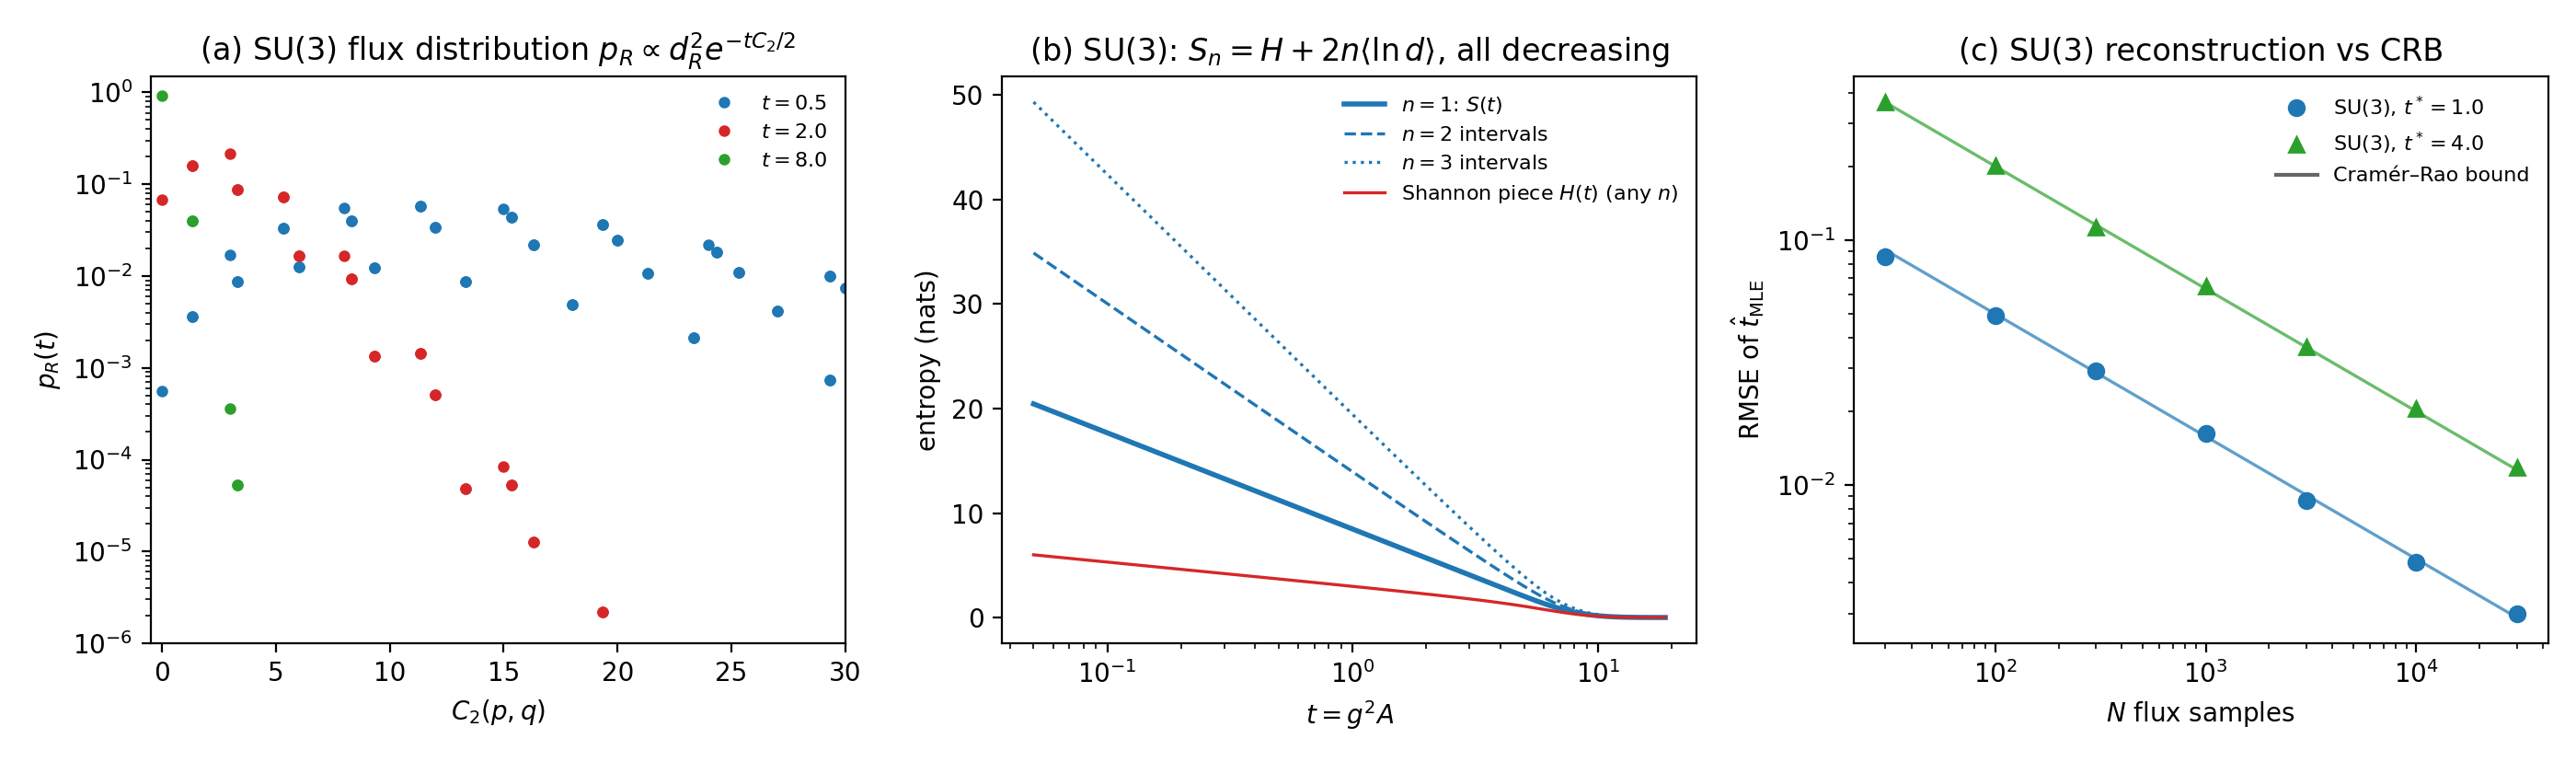
\includegraphics[width=\textwidth]{fig_su3.png}
\caption{$\mathrm{SU}(3)$ and the $n$-interval analysis (script \texttt{ym2\_su3.py}, seed 20260609). (a)~$\mathrm{SU}(3)$ flux distribution over Casimir values at $t \in \{0.5, 2, 8\}$. (b)~$S_n = H + 2n\langle\ln d\rangle$ for $n = 1, 2, 3$ intervals and the $n$-independent Shannon piece $H(t)$: the entropy scales with $n$, the information does not (Sec.~\ref{sec:ncuts}). (c)~$\mathrm{SU}(3)$ reconstruction error versus $N$ against the Cram\'er--Rao bound (Sec.~\ref{sec:qcd}).}
\label{fig:su3}
\end{figure}

\section{Statistical Reconstruction: MLE Against the Cram\'er--Rao Bound}\label{sec:recon}

\textbf{Status: computed (deterministic seed 20260609; $M = 400$ independent batches per point).}

\subsection{Protocol}\label{sec:protocol}

The operational question: an observer who can measure only the gauge-invariant flux observable at one cut draws $N$ i.i.d.\ samples $R_1 \dots R_N$ from $p_R(t^*)$ ($N$ independent preparations; Sec.~\ref{sec:ncuts} is why repeated cuts of one preparation do not count) and estimates $t$. Because \eqref{eq:flux} is an exponential family, the MLE is moment matching --- solve $\langle C_2\rangle_t = N^{-1}\sum_i C_2(R_i)$, which has a unique root since $\langle C_2\rangle_t$ is strictly decreasing by \eqref{eq:cumulant} --- and asymptotic MLE theory guarantees Cram\'er--Rao saturation as $N \to \infty$. The content of the demo is quantitative: \emph{how fast}, at physically interesting $t$, for the groups that matter.

\subsection{Results}\label{sec:results}

At $t^* = 1$ ($M = 400$ trials per cell; RMSE of $\hat t$; $\mathrm{CRB} = \sqrt{1/(N I(t^*))}$; ratio = RMSE/CRB):

\begin{center}
\begin{tabular}{lccccc}
\toprule
group & $I(t^*{=}1)$ & $N = 10^2$ & $N = 10^3$ & $N = 10^4$ & ratio at $10^3$ / $10^4$ \\
\midrule
$\mathrm{U}(1)$ & 0.500 & 0.1437 & 0.0472 & 0.0141 & 1.05 / 1.00 \\
$\mathrm{SU}(2)$ & 1.500 & 0.0800 & 0.0250 & 0.0082 & 0.97 / 1.00 \\
$\mathrm{SU}(3)$ & 4.000 & 0.0490 & 0.0162 & 0.0048 & 1.03 / 0.97 \\
\bottomrule
\end{tabular}
\end{center}

Errors fall as $N^{-1/2}$ along the CR line (Figs.~\ref{fig:ym2}c, \ref{fig:su3}c). Across all $t^* \in \{0.5, 1, 2, 4\}$ at $N = 3\times10^4$: $\Var(\hat t)/\mathrm{CRB} \in [0.93, 1.08]$ ($\mathrm{SU}(2)$, $\mathrm{U}(1)$, 8 cells) and $[0.89, 1.07]$ ($\mathrm{SU}(3)$, 4 cells) --- saturation within Monte-Carlo resolution ($\pm{\sim}7\%$ at 400 trials). Bias is $O(1/N)$ and negligible ($|\mathrm{bias}| \leq 1.4\times10^{-4}$ at $N = 3\times10^4$, $\mathrm{SU}(3)$, $t^* = 1$). $\mathrm{SU}(3)$ reconstruction at $t^* \in \{0.5, 1, 2, 4\}$ and $N = 10^3$ achieves RMSE $\{0.0080, 0.0162, 0.0318, 0.0650\}$, i.e.\ $1.6\%$ relative at $t^* = 1$ and $10^3$ samples, $0.48\%$ at $10^4$. No clamped batches occurred for $\mathrm{SU}(3)$ (the $d_R^2$ degeneracy pressure makes all-trivial-sector samples vanishingly rare); the single pathological batch in the whole series remains the $\mathrm{U}(1)$, $t^* = 4$, $N = 30$ cell documented in the results files.

\subsection{The QCD sentence, and why bigger groups are easier}\label{sec:qcd}

$\mathrm{SU}(3)$ is the gauge group of quantum chromodynamics; the computation above is the statement that \textbf{in the $d = 2$ world, the strong coupling --- the dimensionless $g^2 A$ --- is reconstructible from gauge-invariant entanglement statistics at the Cram\'er--Rao limit.} We confine that sentence to $d = 2$ with the full force of Section~\ref{sec:scope}.

The group-size trend is itself informative. At weak coupling $I(t) \approx \dG/(2t^2)$ (from $C(t) \to \tfrac12\dG$ and \eqref{eq:capacity}): $I(1) = 0.5$, $1.5$, $4.0$ for $\mathrm{U}(1)$, $\mathrm{SU}(2)$, $\mathrm{SU}(3)$. Each flux sample from a larger group carries more information about the coupling, because the Casimir spectrum is richer and the $d_R^2$ degeneracy weighting spreads $p_R$ over more, better-separated sectors. The hierarchy-minded reader of Paper 1 will note the irony: in the one solvable setting, the \emph{non-abelian} couplings are the easy ones.

\subsection{Inversion from the exact entropy}

Independent of sampling: given the exact value of $S(t^*)$ alone (one number, no samples), root-finding on the strictly monotonic $S(\cdot)$ recovers $t^*$ to $\leq 9\times10^{-14}$ at all test points $t^* \in \{0.3, 0.7, 1.5, 3, 6, 12\}$ for all three groups --- the bijection of Proposition~\ref{prop:mono} in practice. We emphasize that this uses the $v = 0$ normalization (Sec.~\ref{sec:groupdata}); an observer uncertain about the additive counterterm should use derivative or sampling data, which are ambiguity-free.

\section{Scope: What This Does and Does Not Show}\label{sec:scope}

\textbf{Status: the deflationary half of the thesis; literature-verified where cited.}

\begin{enumerate}

\item \textbf{It is $d = 2$, and the solvability is the unrepresentativeness.} There are no propagating gluons; the entire entropy is the edge/center term (the distillable term of \cite{D11} vanishes identically). The features that make the theorem exact --- one global flux variable, no transverse physics, area-only dynamics --- are precisely the features absent in $d = 4$. Nothing here is evidence that $d = 4$ couplings live in entanglement; it is the exact statement of what the best case looks like.

\item \textbf{The carrier of the signal is contested as ``entanglement.''} The edge term is non-distillable and drops out of mutual information and relative entropy in the continuum limit \cite{ST16, MST18}; it depends on the choice of center/boundary algebra \cite{CHR}; and although the edge-mode reading has independent support --- it matches the contact term of Kabat \cite{K95} in the Maxwell case \cite{DW14, DW16} --- Casini--Huerta--Mag\'an--Pontello \cite{CHMP} argue that in $d = 4$ Maxwell theory the analogous edge assignment is regularization-dependent, with the physical (anomaly-restoring) effect coming from charged vacuum fluctuations --- an effect \emph{independent of the coupling's value}. Our reconstruction reads information out of exactly the term whose physical status is the live dispute. Two mitigations, honestly weighed: (i) the flux distribution $p_R(t)$ itself is an unambiguous, gauge-invariant object whatever one calls its Shannon entropy --- the statistical reconstruction of Sec.~\ref{sec:recon} needs only $p_R$, not an entropy interpretation; (ii) but an operationalist who insists on distillable entanglement as the only physical entanglement will say this paper reconstructs the coupling from \emph{superselection-sector statistics}, not from entanglement. We think that reading is defensible and the title's ``entanglement statistics'' should be heard with that asterisk.

\item \textbf{Only $g^2 A$ is recoverable --- reflection has a gauge orbit of its own.} By area-preserving diffeomorphism invariance, $g^2$ and $A$ enter all observables only through $t = g^2 A$ \cite{GS14}; ``the coupling'' is recoverable only relative to a fixed fiducial area. This is the $d = 2$ echo of the $d = 4$ obstruction that for noncompact free Maxwell, $g$ can be removed entirely by field redefinition: couplings are scheme-relative quantities, and entanglement data can at best pin down their invariant combinations.

\item \textbf{Reflection, not determination --- the precise statement.} What is proven: the map $t \mapsto p(t)$ is injective (Proposition~\ref{prop:mono}) and its inversion from samples is statistically efficient (Sec.~\ref{sec:recon}). What is presupposed: the group $G$, the Hartle--Hawking preparation, and the functional form of the family \eqref{eq:flux} --- i.e., the entire theory up to one number. An inference of this shape can never show that couplings \emph{are} entanglement properties; it shows that a known theory's coupling leaves a complete, efficiently readable fingerprint in invariant data. Determination would require, at minimum, an induced-coupling framework in which $1/g^2$ is \emph{defined} by an entanglement functional (the gauge analog of Sakharov/Jacobson induced gravity, flagged as unclaimed territory in the series synthesis) --- no such framework exists in the literature we verified.

\item \textbf{The additive ambiguity is real but quarantined.} $S(t)$ carries the $t$-independent counterterm ambiguity (Sec.~\ref{sec:groupdata}). All reconstruction channels used here --- $p_R(t)$, $t$-derivatives of $S$, sampled fluxes --- are ambiguity-free. A claim that needed the absolute value of $S$ would not be.

\end{enumerate}

\section{What \texorpdfstring{$d = 3$ and $d = 4$}{d = 3 and d = 4} Would Require}\label{sec:d34}

\textbf{Status: literature-verified program statement; nothing here is solvable by the methods of this paper.}

\textbf{$d = 3$.} The entropy is no longer all edge: the distillable term of \cite{D11} is nonzero (a propagating photon/gluon), and the boundary flux becomes a \emph{field} on the entangling curve rather than one label. Radi\v{c}evi\'c's weak-coupling analysis \cite{R15} shows the coupling still enters a universal term, $\tfrac12\dG\cdot\log(e^2 r)$ for a region of size $r$ --- formally the same $\tfrac12\dG\cdot\log(\text{coupling})$ structure as our weak-coupling $S(t)$. A $d = 3$ reconstruction program would need: (i) the joint distribution of boundary fluxes (at weak coupling a Gaussian field with covariance $\langle E_\perp E_\perp\rangle$ set by $e^2$) --- note that unlike our single global $R$, \emph{this} distribution genuinely has more independent components for larger boundaries, so the $n$-cuts no-go of Sec.~\ref{sec:ncuts} is a $d = 2$ peculiarity, not a general law; (ii) separation of the universal log coefficient from non-universal perimeter pieces; (iii) a stance on the center choice, which in $d \geq 3$ affects the sufficient statistics themselves \cite{CHR}.

\textbf{$d = 4$.} Three verified facts frame the problem. (i) For noncompact free Maxwell, vacuum entanglement cannot depend on $g$ at all (field redefinition). (ii) For compact $\mathrm{U}(1)$, the coupling enters through flux-sector (zero-mode) weights --- a finite, topological term \cite{DW16} --- and through compactness effects on the edge partition function; this is the closest $d = 4$ analog of our $p_R(t)$ and the natural first target: \emph{the flux-sector distribution on a compact entangling surface is an exponential family in $1/e^2$ with sufficient statistic the flux quantum number squared}, and a Fisher analysis of it would be a direct (if much weaker) descendant of Sec.~\ref{sec:fisher}. (iii) With charged matter, the one sharp computation \cite{CHMP} finds the log-coefficient shift universal --- independent of the coupling's value and of the charge masses. So in $d = 4$ the live possibilities are: the coupling enters only through compactness/topology (reconstructible but topological, not local), or only through scale-dependence of coarse-grained flux statistics (the ``reconstruction, not identification'' conjecture of the series synthesis), or not at all in any distillable quantity. Deciding among these is the open problem the series hands to whoever next enters; the $d = 2$ result fixes the gold standard such a program should be measured against --- exponential-family structure, identity \eqref{eq:dSisI}, CR saturation --- while its own $n$-cuts lesson warns that gauge theories can manufacture arbitrarily much edge entropy carrying zero additional information.

\section{Conclusion: The Series Closed Into a Point}

Paper 1 proved that the frame-dependent version of ``couplings from entanglement'' is ill-posed and that its static matchings are non-evidential. Paper 2 made the question well-posed with the algebraic (commutant/center) definition and showed that in the minimal toy the well-posed answer is a sharper no-go --- and that all gauge-invariant entanglement there is, is the classical edge term. This paper went to the one place where that edge term is an exactly solvable function of a gauge coupling and extracted everything it contains: the coupling is reflected \emph{completely} (bijection), \emph{identifiably} (one global flux variable, with no information inflation from extra cuts), and \emph{efficiently} (Cram\'er--Rao saturation, for $\mathrm{U}(1)$, $\mathrm{SU}(2)$, and the QCD group $\mathrm{SU}(3)$, with larger groups easier). The exact identities
\[
\frac{dS}{dt} = -\frac{t}{4}\Var_t(C_2) = -t\,I(t) = -\frac{C(t)}{t}
\]
say in one line what the series learned the long way: in $d = 2$, entanglement susceptibility, flux susceptibility, Fisher information, and capacity of entanglement are one function, and that function knows the coupling.

What none of this shows is determination. The inference presupposes the theory; the recovered number is the scheme-invariant product $g^2 A$; the carrier is a term whose entanglement credentials are contested; and the $d = 4$ evidence is, if anything, adverse. The honest summary of the series is therefore a conditional: \emph{if} gauge couplings are encoded in vacuum entanglement in the actual world, the encoding must be of the kind exhibited here --- gauge-invariant flux statistics, not frame-dependent subsystem entropies --- and whether any $d = 4$ version of that encoding exists, beyond topological zero modes, is the open question. The no-gos cleared the ground; this paper is the one building that provably stands on it; everything taller is future work, and we have priced the lumber.

\appendix

\section{Reproducibility}

All computations are deterministic (seed 20260609) and complete in seconds on a laptop. Repository layout (paths relative to repo root):

\begin{itemize}
\item \texttt{ym2/FORMULAS.md} --- every literature formula with citation and verbatim source string, verified against the arXiv LaTeX of \cite{D14}, \cite{GS14}, \cite{D11} (fetched 2026-06-09); the convention discrepancies found (\cite{GS14} Casimir $\times 2$; additive counterterm) and resolutions.
\item \texttt{ym2/ym2\_flux.py} --- $\mathrm{U}(1)$ and $\mathrm{SU}(2)$: curves, monotonicity, inversion, MLE/CRB demo. Output: \texttt{results.json}, \texttt{fig\_ym2.png/.pdf} (Fig.~\ref{fig:ym2}). Runtime ${\approx}8$ s.
\item \texttt{ym2/ym2\_su3.py} --- \textbf{new for this paper.} $\mathrm{SU}(3)$ (convention asserted at runtime on the irreps $\mathbf{1}$, $\mathbf{3}$, $\bar{\mathbf{3}}$, $\mathbf{6}$, $\mathbf{8}$, $\mathbf{10}$), plus the $n$-interval analysis for all three groups: identity \eqref{eq:dSndt} by central differences, and the Fisher non-scaling demonstration. Output: \texttt{su3\_results.json}, \texttt{fig\_su3.png/.pdf} (Fig.~\ref{fig:su3}). Runtime ${\approx}3$ s. Run \texttt{python3 ym2\_su3.py} (no arguments) for the full pipeline; staged execution (\texttt{stage1}, \texttt{stage2:0.5,1.0}, \texttt{stage2:2.0,4.0}, \texttt{stage3}, \texttt{merge}) produces bit-identical results via per-component RNG streams \texttt{default\_rng([SEED, stage, index])}.
\item Truncation policy: curve/identity computations keep all irreps with relative weight $> e^{-800}$ (truncation error exactly zero in float64); the MLE inner loop uses $e^{-120}$ (relative truncation $< 10^{-50}$, ${\sim}46$ orders below Monte-Carlo noise). For $\mathrm{SU}(3)$ the irrep sum runs over a $(p,q)$ grid with $p, q \leq \sqrt{6 \cdot 860 / t} + 2$.
\item Headline residuals: $|S_{\text{direct}} - S_{\text{exponential-family}}| \leq 3.6\times10^{-15}$ ($\mathrm{SU}(3)$, 400 grid points); identity \eqref{eq:dSndt} to $2.4\times10^{-10}$ (48 combinations); inversion $\leq 9\times10^{-14}$ (18 test points); capacity plateau $\tfrac12\dG$ to $< 10^{-6}$ at $t = 0.05$.
\end{itemize}

\begin{thebibliography}{99}

\bibitem{P1} W. T. Trevena, ``Is the Standard Model Coupling Hierarchy Encoded in Three-Qubit Vacuum Entanglement? No-Go Results, an Exact Octonionic Vacuum, and the Surviving Hypothesis Space,'' companion paper (2026), repository \texttt{paper/draft.md}.

\bibitem{P2} W. T. Trevena, ``Gauge-Invariant Entanglement in a Minimal Fermionic Toy: The Coupling--Entropy Question Made Well-Posed --- and Closed,'' companion paper (2026), repository \texttt{paper2/sequel\_draft.md}.

\bibitem{Mig75} A. A. Migdal, ``Recursion equations in gauge field theories,'' Sov. Phys. JETP 42, 413 (1975).

\bibitem{Rus90} B. Rusakov, ``Loop averages and partition functions in U(N) gauge theory on two-dimensional manifolds,'' Mod. Phys. Lett. A5, 693 (1990).

\bibitem{Wit91} E. Witten, ``On quantum gauge theories in two dimensions,'' Commun. Math. Phys. 141, 153 (1991).

\bibitem{CMR94} S. Cordes, G. Moore, and S. Ramgoolam, ``Lectures on 2D Yang--Mills theory, equivariant cohomology and topological field theories,'' Nucl. Phys. B Proc. Suppl. 41, 184 (1995); arXiv:hep-th/9411210.

\bibitem{D11} W. Donnelly, ``Decomposition of entanglement entropy in lattice gauge theory,'' Phys. Rev. D 85, 085004 (2012); arXiv:1109.0036.

\bibitem{D14} W. Donnelly, ``Entanglement entropy and nonabelian gauge symmetry,'' Class. Quantum Grav. 31, 214003 (2014); arXiv:1406.7304.

\bibitem{GS14} A. Gromov and R. A. Santos, ``Entanglement entropy in 2D non-abelian pure gauge theory,'' Phys. Lett. B 737, 60 (2014); arXiv:1403.5035.

\bibitem{V08} A. Velytsky, ``Entanglement entropy in d+1 SU(N) gauge theory,'' Phys. Rev. D 77, 085021 (2008); arXiv:0801.4111.

\bibitem{CHR} H. Casini, M. Huerta, and J. A. Rosabal, ``Remarks on entanglement entropy for gauge fields,'' Phys. Rev. D 89, 085012 (2014); arXiv:1312.1183.

\bibitem{GST15} S. Ghosh, R. M. Soni, and S. P. Trivedi, ``On the entanglement entropy for gauge theories,'' JHEP 09 (2015) 069; arXiv:1501.02593.

\bibitem{ST16} R. M. Soni and S. P. Trivedi, ``Entanglement entropy in (3+1)-d free U(1) gauge theory,'' JHEP 02 (2017) 101; arXiv:1608.00353.

\bibitem{MST18} U. Moitra, R. M. Soni, and S. P. Trivedi, ``Entanglement entropy, relative entropy and duality,'' JHEP 08 (2019) 059; arXiv:1811.06986.

\bibitem{DW14} W. Donnelly and A. C. Wall, ``Entanglement entropy of electromagnetic edge modes,'' Phys. Rev. Lett. 114, 111603 (2015); arXiv:1412.1895.

\bibitem{DW16} W. Donnelly and A. C. Wall, ``Geometric entropy and edge modes of the electromagnetic field,'' Phys. Rev. D 94, 104053 (2016); arXiv:1506.05792.

\bibitem{CHMP} H. Casini, M. Huerta, J. M. Mag\'an, and D. Pontello, ``On the logarithmic coefficient of the entanglement entropy of a Maxwell field,'' Phys. Rev. D 101, 065020 (2020); arXiv:1911.00529.

\bibitem{K95} D. Kabat, ``Black hole entropy and entropy of entanglement,'' Nucl. Phys. B 453, 281 (1995); arXiv:hep-th/9503016.

\bibitem{R15} \DJ. Radi\v{c}evi\'c, ``Entanglement in weakly coupled lattice gauge theories,'' JHEP 04 (2016) 163; arXiv:1509.08478.

\bibitem{BMV18} A. Blommaert, T. G. Mertens, and H. Verschelde, ``Edge dynamics from the path integral: Maxwell and Yang--Mills,'' JHEP 11 (2018) 080; arXiv:1804.07585.

\bibitem{DTV19} W. Donnelly, S. Timmerman, and N. Vald\'es-Meller, ``Entanglement entropy and the large N expansion of two-dimensional Yang--Mills theory,'' JHEP 04 (2020) 182; arXiv:1911.09302.

\bibitem{MOPT26} D. Melnikov, J. T. Oliveira, V. Peixoto, and M. Tenser, ``States of 2D Yang--Mills and large-volume entanglement,'' arXiv:2603.10171 (2026).

\bibitem{ASV24} R. Amorosso, S. Syritsyn, and R. Venugopalan, ``Entanglement entropy of a color flux tube in (1+1)D Yang--Mills theory,'' arXiv:2411.12818; ``Entanglement entropy of a color flux tube in (2+1)D Yang--Mills theory,'' JHEP 12 (2024) 177; arXiv:2410.00112.

\bibitem{YQ10} H. Yao and X.-L. Qi, ``Entanglement entropy and entanglement spectrum of the Kitaev model,'' Phys. Rev. Lett. 105, 080501 (2010); arXiv:1001.1165.

\bibitem{dBJK18} J. de Boer, J. J\"arvel\"a, and E. Keski-Vakkuri, ``Aspects of capacity of entanglement,'' Phys. Rev. D 99, 066012 (2019); arXiv:1807.07357.

\bibitem{N21} P. Nandy, ``Capacity of entanglement in local operators,'' JHEP 07 (2021) 019; arXiv:2106.00228.

\bibitem{GS18} M. Goldstein and E. Sela, ``Symmetry-resolved entanglement in many-body systems,'' Phys. Rev. Lett. 120, 200602 (2018); arXiv:1711.09418.

\bibitem{XAS18} J. C. Xavier, F. C. Alcaraz, and G. Sierra, ``Equipartition of the entanglement entropy,'' Phys. Rev. B 98, 041106(R) (2018); arXiv:1804.06357.

\bibitem{ADKT23} R. Arias, G. Di Giulio, E. Keski-Vakkuri, and E. Tonni, ``Probing RG flows, symmetry resolution and quench dynamics through the capacity of entanglement,'' JHEP 03 (2023) 175; arXiv:2301.02117.

\bibitem{BC94} S. L. Braunstein and C. M. Caves, ``Statistical distance and the geometry of quantum states,'' Phys. Rev. Lett. 72, 3439 (1994).

\bibitem{Cam90} R. Camporesi, ``Harmonic analysis and propagators on homogeneous spaces,'' Phys. Rep. 196, 1 (1990).

\bibitem{su3data} Standard sources for $\dim(p,q) = (p+1)(q+1)(p+q+2)/2$ and $C_2(p,q) = (p^2+q^2+pq+3p+3q)/3$: e.g.\ A. B. Balantekin et al., lecture notes, arXiv:2109.12087; H. Georgi, \emph{Lie Algebras in Particle Physics}, 2nd ed., Westview Press (1999); Wikipedia, ``Clebsch--Gordan coefficients for SU(3)'' (accessed 2026-06-09). Verified to satisfy $C_2(1,0) = (N^2-1)/2N$ and $C_2(1,1) = N$; asserted at runtime in \texttt{ym2\_su3.py}.

\bibitem{BKOV} H. Barnum, E. Knill, G. Ortiz, and L. Viola, ``Generalizations of entanglement based on coherent states and convex sets,'' Phys. Rev. A 68, 032308 (2003); arXiv:quant-ph/0305023.

\bibitem{Zanardi} P. Zanardi, ``Virtual quantum subsystems,'' Phys. Rev. Lett. 87, 077901 (2001); arXiv:quant-ph/0103030.

\end{thebibliography}

\end{document}
